\chapter{Renewal Theory and Some Applications}
\label{ren}

Remember the light bulb example in Section \ref{expon}?  You may be
startled to learn that entire books have been written on a
generalization of that example.  This chapter will just scratch the
surface of the important topic.

\section{Introduction} 

\subsection{The Light Bulb Example, Generalized}
 
Supposre a certain lamp is used continuously, and that whenever its bulb
burns out, it is immediately replaced by a new one. Let N(t) denote the
number of replacements, called \textbf{renewals} here, that have
occurred up through time t. Assume the lifetimes of the bulbs, \(
L_{1},\, L_{2,}\, L_{3,}\, ...$ are independent and identically
distributed. The collection of random variables $N(t), t\geq 0$ is
called a \textbf{renewal process.}  The quantities $R_{i} = L_1+...+L_i$
are called the {\bf renewal points}.

We will see that most renewal processes are not Markovian.  However,
time does ``start over'' at the renewal points.  We say the process is
{\bf regenerative} at these points.

Note that although we are motivating this with the lightbulb example,
in which the $L_{i}$ measure time, the theory we will present here
is not limited to such a context. All that is needed is that the \(
L_{i}$ be i.i.d. and nonnegative.

There is a very rich collection of mathematical material on renewal
processes, and there are myriad applications to a variety of fields.

\subsection{Duality Between ``Lifetime Domain'' and ``Counts Domain''}
\label{domains}

A very important property of renewal processes is that

\begin{equation}
\label{equivdoms}
N(t) \geq k  \textrm{ if and only if } R_k \leq t
\end{equation}

This is just a formal mathematical of common sense:  There have been at
least k renewals by now if and only if the $k^{th}$ renewal has already
occurred!  But it is a very important device in renewal analysis.

Equation (\ref{equivdoms}) might be described as relating the ``counts
domain'' (left-hand side of the equation) to the ``lifetimes domain''
(right-hand side).

\section{Where We Are Going}

Some of the material in Sections \ref{pois} and \ref{renprops} of this 
chapter may seem a little theoretical.  However, it all does have practical
value, and it will also exercise some of the concepts you've learned in
earlier chapters.  

After those two sections, the focus will mainly be on concepts which
apply the theory, and on specific examples.

\section{Properties of Poisson Processes}
\label{pois}

\subsection{Definition}

A renewal process N(t) is called a \textbf{Poisson process} if each N(t)
has a Poisson distribution, i.e. for some $\lambda $ we have

\begin{equation}
P(N(t)=k)=\frac{e^{-\lambda t}(\lambda t)^{k}}{k!},\, k=0,1,2,3,...
\end{equation}

The parameter $\lambda $ is called the \textbf{intensity parameter}
of the process, and since $E[N(t)]=\lambda t$, it has the natural
interpretation of the (average) rate at which renewal events occur per
unit time.

\subsection{Alternate Characterizations of Poisson Processes}

\subsubsection{Exponential Interrenewal Times}

\begin{theorem}

A renewal process N(t) is a Poisson process if and only if the
interrenewal times $L_{i}$ have an exponential distribution with
parameter $\lambda $.  

Note that this shows that a Poisson process is also a Markov chain (with
state being the current number of renewals), due to the memoryless
property of the exponential distribution.

\end{theorem}

\begin{proof}

For the ``only if'' part of the claim, note that from the ``domain
switching'' discussed in Section (\ref{domains}), 

\begin{equation}
F_{L_{1}}(t)=1-P(L_{1}>t)=1-P(N(t)=0)=1-e^{-\lambda t}
\end{equation}

Differentiating with respect to t, we find that $f_{L_{1}}(t)=\lambda
e^{-\lambda t}$.  Since the $L_i$ are i.i.d. by definition of renewal
proceses, this shows that all the $L_i$ have an exponential
distribution.

\end{proof}

\subsubsection{Stationary, Independent Increments}

\begin{theorem}

Suppose N(t) is a renewal process for which the $L_i$ are
continuous random variables.

Then N(t) is a Poisson process if and only if it has \textbf{stationary,
independent increments}.  The latter term means that for all 
$0<r<s<t<u$ we have the following properties: 

\begin{itemize}

\item [(a)] Independent increments:  N(s)-N(r) and N(u)-N(t) are
independent random variables.

\item [(b)] Stationarity:  The distribution of N(s)-N(r) is the same as
that of N(s+z)-N(r+z) for any z $>$ 0.

\end{itemize}

\end{theorem}

\begin{proof}

(Sketch.)

For the ``only if'' part:  As noted above, Poisson processes have the
Markov property, which immediately implies independent increments.
Also, since ``time starts over,'' say at time r, then for s $>$ r we
will have that N(s) - N(r) has the same distribution as N(s-r).

For the ``if'' part:  The independence of the increments implies the
Markov property, and since the only continuous distribution which is
memoryless is the exponential, that implies the the $L_i$ have
exponential distributions, which we saw above implies that N(t) is
Poisson.

\end{proof}

Note too that for these reasons N(s)-N(r) will have the same
distribution as N(s-r).

We can use these properties to find the {\bf autocorrelation function}
of the Poisson process, which shows the correlation of the process with
itself at different times $s < t$:

\begin{equation}
c(s,t) = \frac{Cov[N(s),N(t)]}
{\sqrt{Var[N(s)] Var[N(t)]}}
\end{equation}

To derive this quantity, note first that

\begin{eqnarray}
E[N(s)N(t)] &=& E\left[N(s) \{N(t)-N(s)\} + N^2(s)\right]~~~~
   \textrm{(algebra)} \\ 
&=& E\left[N(s) \{N(t)-N(s)\}\right] + E\left[N^2(s)\right] ~~~~
   \textrm{(E is lin.)} \\
&=& E[N(s)] E[N(t)-N(s)] + E\left[N^2(s)\right] ~~~~
   \textrm{(indep. incs.)} \\
&=& [\lambda s \cdot \lambda (t-s)] + [\lambda s + (\lambda s)^2] ~~~~
   \textrm{(Pois., $(\ref{varuformula})$}
\end{eqnarray}

% \checkpoint

Here we used the property of independent increments in going from the
second to third line.  In the last line we have used the fact that N(u)
has mean and variance both equal to $\lambda u$ for all $u > 0$.

After performing the remaining calculations, we find that

\begin{equation}
c(s,t) = \sqrt{\frac{s}{t}}
\end{equation}

\subsection{Conditional Distribution of Renewal Times}

\begin{theorem}

Suppose N(t) is a Poisson process.  Let $R_i = L_1+...+L_i$ be the
renewal times, i = 1,2,3,...

Given N(t) = k, then $M_{1},...,M_{k}$ are i.i.d. U(0,t) (uniform
distribution on (0,t)), where the $(M_1,...,M_k)$ is a random
permutation of $(R_1,...,R_k)$.  

In other words, conditional on there being k renewals within (0,t), the
unordered renewal times are independent and uniformly distributed on
(0,t).  

\end{theorem}

This fact often plays a key role in analyses of Poisson models.

Let's look at the intuitive meaning of this, using our ``notebook''
view, taking k = 3 and t = 12.0 for concreteness.

Each line of the notebook would consist of the results of our observing
the process up to time 12.0.  The first column would show the $R_1$, the
second $R_2$ and so on.

We would also have columns for $M_1$, $M_2$ and $M_3$.  These would be
filled with NAs (``not applicable'') in rows for which N(12.0) is not
equal 3, while in rows for which N(12.0) {\it is} equal to 3,
$(M_1,M_2,M_3)$ would be a random scrambling of $(R_1,R_2,R_3)$.  

The uniform distribution part of the theorem is saying that among the
rows in which N(12,0) = 3, 1/2 of them will have, for instance, $M_1 <
6.0$.  That will NOT be true for $R_1$; considerably fewer than 1/2 of
the rows will have $R_1 < 6.0$.  The independence part of the theorem is
saying, for example, that 1/4 of these rows will have {\it both} $M_1 <
6.0$ {\it and} $M_2 < 6.0$.

Here's the proof.

\begin{proof}

Let Y denote the number of $M_i \leq s$.  Then 

\begin{eqnarray}
P(Y = b | N(t) = k) &=& 
\frac
{P(Y = b ~{\rm and}~ N(t) = k)}
{P[N(t) = k]} \\ 
&=& 
\frac
{P[N(s) = b ~{\rm and}~ N(t)-N(s) = k-b]}
{P[N(t) = k]} \\ 
&=&
\frac
{
   {\frac{e^{-\lambda s}(\lambda s)^b}{b!}} \cdot
   {\frac{e^{-\lambda (t-s)} (\lambda (t-s))^{k-b}}{(k-b)!}}
}
{
   \frac
      {e^{\lambda t} (\lambda t)^k}
      {k!}
} \\
&=& \binom{k}{b} {(\frac{s}{t})}^b {(1-\frac{s}{t})}^{k-b}
\end{eqnarray}

This is the probability that would arise if the $M_i$ were i.i.d. U(0,t)
as claimed in the theorem.

% While not proving this in general, let us consider the case k = 1:
% 
% \begin{eqnarray}
% P(L_{1}<s|N(t)=1) & = & \frac{P(L_1 < s \textrm{ and } N(t)=1)} {P(N(t)=1)}
% \nonumber \\
% & = & \frac{P(N(s)=1\textrm{ and }N(t)-N(s)=0)} {P(N(t)=1)}
% \nonumber \\
% & = & \frac{P(N(s)=1)P(N(t)-N(s)=0)}
% {P(N(t)=1)} 
% \nonumber \\
% & = & \frac
% { \left [ e^{-\lambda s}{[\lambda s]}^1/1! \right ]  
% \left [ e^{-\lambda (t-s)}{(\lambda (t-s))}^0/0! \right ] }
% {e^{-\lambda t}{(\lambda t)}^1/1!} \nonumber \\
% & = & \frac{s}{t}
% \end{eqnarray}
% 
% where we have again switched domains as in Section (\ref{domains}) and
% have used the fact that a Poission process has independent increments,
% as noted earlier. Taking the derivative, we then have that the density
% of $L_1$ given N(t) = 1 is the constant 1/t, i.e.  $L_i$ uniformly
% distributed on (0,t).

\end{proof}

\subsubsection{Example:  Message Buildup at a Broken Network Link}

Suppose messages arrive to a network link according to a Poisson
process. Unfortunately, the link is down, and the messages just keep
piling up. Suppose at time 60.0 we see 10 messages in the buffer. Find
the variance of the total wait time of those messages.

{\bf Solution:}  Number the messages 1 through 10, not necessarily in
the order of their arrival.  Say for instance that these messages came
from mouse clicks of 10 Web users, and we order the messages by the
surnames of the users.  That gives us a random permutation of the 10
messages, and since we are only analyzing the total of the 10 wait
times, it doesn't matter which permutation we have.
 
Let $W_1,...,W_{10}$ be the wait times of our 10 messages.  Then,
conditional on N(60.0), the $W_i$ are independent and i.i.d. U(0,60.0).
Then from Section \ref{unifprops}, $EW_i = 30.0$ and $Var(W_i) = 60^2/12
= 300$.  The mean and variance of the total wait time are thus
300 and 3000.

\subsection{Decomposition and Superposition of Poisson Processes}

\begin{theorem}

Poisson processes can be split and combined:

\begin{itemize}

\item [(a)] Let N(t) be a Poisson process with intensity parameter
$\lambda$.  Say we \textbf{decompose} N(t) into $N_{1}(t)$ and
$N_{2}(t)$ by assigning each renewal in N(t) to either $N_{1}(t)$ or
$N_{2}(t)$ with probability p and 1-p respectively.  Then the two
resulting processes are again Poisson processes.  They are independent
of each other, and have intensity parameters $p\lambda $ and
$(1-p)\lambda $. 

\item [(b)] If we \textbf{superimpose} two independent Poisson processes
$N_{1}(t)$ and $N_{2}(t)$, the result $N(t) = N_{1}(t) + N_{2}(t)$
will be a Poisson process, with intensity parameter equal to the sum of
the two original parameters.

\end{itemize}

\end{theorem}

These properties are often useful in queuing models, where an arrival
process is subdivided in two processes corresponding to two job classes.

\subsection{Nonhomogeneous Poisson Processes}

A useful variant of Poisson processes is the {\bf nonhomogeneous Poisson
process}.  The key here is that the intensity parameter $\lambda$ varies
over time.  We will write it as $\lambda(t)$.  I'll define it this way:

\begin{definition} Let $N(t), t\geq 0$ be a counting process with
independent increments, and let  

\begin{equation}
m(t) = E[N(t)]
\end{equation}

If for all $0 < s < t$ we have

\begin{equation}
P[N(t) - N(s) = k] = \frac{e^{-m(t-s)}[m(t-s)[^k}{k!}, k = 0,1,2,...
\end{equation}

then we say that $N(t), t\geq 0$ is a nonhomogeneous Poisson
process with intensity function

\begin{equation}
\lambda(t) = \frac{d}{dt} m(t)
\end{equation}

\end{definition} 

Intuitively, $N(t), t\geq 0$ is a Markov process with states of the form
[t,N(t)].  In that state, the probability that there will be a renewal
in the next $\Delta t$ amount of time is approximately $\Delta t \cdot
\lambda(t)$, for small increments of time $\Delta t$.

\subsubsection{Example:  Software Reliability}

Nonhomogeneous Poisson process models have been used successfully 
to model the ``arrivals'' (i.e. discoveries) of bugs in software.
Questions that arise are, for instance, ``When are we ready to ship?'',
meaning when can we believe with some confidence that most bugs have
been found?

Typically one collects data on bug discoveries from a number of projects
of similar complexity, and estimates m(t) from that data.

See for example Estimating the Parameters of a Non-homogeneous
Poisson-Process Model for Software Reliability, {\it IEEE Transactions
on Reliability, Vol. 42, No. 4, 1993}.

\section{Properties of General Renewal Processes}
\label{renprops}

We now turn our attention to the general case, in which the $L_{i}$ are
not necessarily exponentially distributed. We will still assume the $L_{i}$
to be continuous random variables, though.

\subsection{The Regenerative Nature of Renewal Processes}

Recall that Markov chains are ``memoryless.'' If we are now at time t, ``time
starts over,'' and the probabilities of events after time t do not depend on
what happened before time t.

If the $L_{i}$ are not exponentially distributed, N(t) is not
Markovian, since the exponential distribution is the only continuous
memoryless distribution.  However, it is true that ``time starts over'' at
each renewal epoch $R_i = L_1+...+L_i$.  Note the difference: The
definition of the Markov property concerns time starting over at a fixed
time, t. Here, in the context of renewal processes, ``time starts over''
at random times, of the form $R_i$.

\subsection{Some of the Main Theorems}

Let m(t) = E{[}N(t){]}. Many of the results concern this function m. 
Please forgive a bit of abuse of notation:

\begin{equation}
F = F_L
\end{equation}

\begin{equation}
f = f_L
\end{equation}

\begin{equation}
F_n = F_{R_n}
\end{equation}

\subsubsection{The Functions $F_n$ Sum to m}

First, we need a general property of means of nonnegative random
variables (this was an exercise in Chapter 1):

\begin{lemma}
\label{reverse}

For any nonnegative-integer valued random variable Z,

\begin{equation}
E(Z) = \sum ^{\infty }_{j=1}P(Z\geq j) 
= \sum ^{\infty }_{j=0} [1 - F_Z(j)]
\end{equation}

If Z is a nonnegative continuous random variable, then

\begin{equation}
E(Z) 
= \int ^{\infty }_{0} [1 - F_Z(t)] ~ dt
\end{equation}

\end{lemma}

\begin{proof}

In the discrete case,

\begin{eqnarray}
E(Z) & = & \sum ^{\infty }_{i=1}i\, P(Z=i) \\
 & = & \sum ^{\infty }_{i=1}P(Z=i)\, \sum ^{i}_{j=1}1\\
 & = & \sum ^{\infty }_{j=1}\, \sum ^{\infty }_{i=j}P(Z=i)\\
 & = & \sum ^{\infty }_{j=1} P(Z\geq j) \\
 & = & \sum ^{\infty }_{j=0} P(Z > j) \\
 & = & \sum ^{\infty }_{j=0} [1 - F_Z(j)]
\end{eqnarray}

The continuous case is similar.

\end{proof}

Now, let's apply that:

\begin{theorem}

\begin{equation}
\label{mfn}
m(t)=\sum ^{\infty }_{n=1}F_{n}(t)
\end{equation}

\end{theorem}

\begin{proof}

Let Z = N(t). Then yet again switching domains as in Section
(\ref{domains}),

\begin{equation}
m(t)=\sum ^{\infty }_{j=1}P(N(t)\geq j)=\sum ^{\infty
}_{j=1}P(R_{j}\leq t)=\sum ^{\infty }_{j=1}F_{j}(t)
\end{equation}

\end{proof}

\subsubsection{The Renewal Equation}

\begin{theorem}

The function m satisfies the equation

\begin{equation}
\label{reneweqn}
m(t) = F(t)+\int _{0}^{t}m(t-w)\, f(w)\, dw
\end{equation}

\end{theorem}

\begin{proof}


Using the Law of Total Expectation, we have

\begin{equation}
\label{thatlawagain}
m(t)=E[N(t)]=E\{E[N(t)|L_{1}]\}
\end{equation}

But at time $L_{1}$ ``time starts over again,'' by the regenerative
property of renewal processes. So,

\begin{equation}
E[N(t)|L_{1})=\left\{ \begin{array}{rl}
1+m(t-L_{1}), & \textrm{if }L_{1}<t\\
0, & \textrm{otherwise}
\end{array}\right. 
\end{equation}

Remember, $E[N(t)|L_{1})$ is a function of $L_1$.  Thus its expected
value, which we want to find now (see (\ref{thatlawagain})), is the
integral of that function times the density of $L_1$:

\begin{equation}
m(t)=\int _{0}^{t}[1+m(t-w)]\, f(w)\, dw=F(t)+\int _{0}^{t}m(t-w)\, f(w)\, dw
\end{equation}

% \checkpoint

\end{proof}

If f is known, then F is known too, then  Equation (\ref{reneweqn}) can be
solved for m.  This is known as an \textbf{integral equation} for m,
analogous to a differential equation.  In fact, it can be converted to a
differential equation by taking the derivative of both sides. There are
various techniques for solving integral equations, including numerical
approximations, but we will not pursue those here.

The function m is useful in a number of contexts (one of which will be
seen in Section \ref{ross}), so we will now look at some of its
properties.

\subsubsection{The Function m(t) Uniquely Determines F(t)}

Remember, each different distribution for the $L_i$ gives rise to a
different distribution for the N(t), thus a different m(t).  The
converse is also true:

\begin{theorem}
The function m(t) uniquely determines F(t).
\end{theorem}

\begin{proof}

For any function h (for which the absolute value has a finite integral
on $(0,\infty )$), let $\Lambda _{h}$ define the Laplace transform of h,

\begin{equation}
\Lambda _{h}(s)=\int ^{\infty }_{0}e^{-st}h(t)\, dt
\end{equation}

Now, we will take the Laplace transform of both sides of (\ref{reneweqn}).
To do so, we will need to state some facts about Laplace transforms.

Remember, Laplace transforms are, except for a change of variable, just
like generating functions or moment generating functions, which you
probably studied in your undergraduate probability course. Thus Laplace
transforms have the same properties as generating functions.

Now recall that the generating function of the sum of two independent
nonnegative random variables is the product of their individual moment
generating functions. Well, the density of such a sum has the same
integral form as in (\ref{reneweqn}), which we call a
\textbf{convolution.} Even though the m part of the integral is not a
density function, it is still true that the Laplace transform of a
convolution of two functions is the product of their individual Laplace
transforms.

So, taking the Laplace transform of both sides of (\ref{reneweqn}) yields:

\begin{equation}
\Lambda _{m}(s)=\Lambda _{F}(s)+\Lambda _{m}(s)\Lambda _{f}(s)
\end{equation}

i.e.

\begin{equation}
\Lambda _{m}(s)= \frac{\Lambda _{F}(s)} {1-\Lambda _{f}(s)}
\end{equation}

This says that m uniquely determines the Laplace transforms of $F_{}
\) and $f$, and since there is a one-to-one correspondence between
distributions and Laplace transforms, we see that m uniquely determines
the interrenewal distribution.  In other words, there is only one
possible interrenewal distribution for any given mean function.

\end{proof}

In fact, some similar analysis, which we will not present here, yields:

\begin{equation}
\label{notpresent}
\Lambda _{f}(s)=\frac{\Lambda _{r}(s)}{1+\Lambda _{r}(s)}
\end{equation}

where $r(t)=\frac{d}{dt}m(t)$.   So, we can recover f from m.

As an example, we earlier saw that there are three equivalent
definitions of a Poisson process, i.e. each implies the other. We can
use the above result to show one of those equivalences:

Suppose a renewal process has stationary, independent increments. This
would imply that m(t) = ct for some c $>$ 0, and thus r(t) = c. Then

\begin{equation}
\Lambda _{r}(s)=\int ^{\infty }_{0}e^{-st}c\, dt=\frac{c}{s}
\end{equation}

so (\ref{notpresent}) gives us

\begin{equation}
\Lambda _{f}(s)=\frac{c}{s+c}
\end{equation}

This is the Laplace transform for the exponential distribution with
parameter c. So, we see how the stationary, independent increments
property implies exponential interrenewal times.


\subsubsection{Asymptotic Behavior of m(t)}

\begin{theorem}

\begin{equation}
\label{key}
\lim_{t\rightarrow \infty }\frac{m(t)}{t}=\frac{1}{E(L)}
\end{equation}

\end{theorem}

This should make good intuitive sense to you.  By the way, this (and
some other things we'll find in this chapter) can be used to formally prove
some assertions we made on only an intuitive basis in early chapters.

\section{Alternating Renewal Processes}

\subsection{Definition and Main Result}

Suppose we have a sequence of pairs of random variables $(Y_{n},Z_{n})
\) which are i.i.d. \textit{as pairs}. In other words, for instance the
pair $(Y_{1},Z_{1})$ is independent of, but has the same
distribution as, $(Y_{2},Z_{2})$ and so on, but on the other hand \(
Y_{n}$ and $Z_{n}$ are allowed dependency. 

Imagine a machine being busy, then idle, then busy, then idle, and so
on, with $Y_{n}$ being the amount of ``on'' time in the $n^{th}$ cycle,
and similarly $Z_{n}$ being the ``off'' time. Each time an on/off
pair finishes, call that a ``renewal.'' The sequence is called an
\textbf{alternating renewal process}. 

It is intuitively clear, and can be proven, that

\begin{equation}
\label{alton}
\lim_{t\rightarrow \infty }P(\textrm{on at time t})=\frac{E(Y)}{E(Y)+E(Z)}
\end{equation}

and 
\begin{equation}
\label{altoff}
\lim_{t\rightarrow \infty }P(\textrm{off at time t})=\frac{E(Z)}{E(Y)+E(Z)}
\end{equation}

Again, these results can be used to formally prove some assertions we
have made in earlier chapters on just an intuitive basis.

\subsection{Example:  Inventory Problem (difficult)}
\label{ross}

(Adapted from \textit{Stochastic Processes}, by Sheldon Ross, Wiley, 1996.)

Consider a vendor which uses an \textbf{(s,S) policy} for replenishing
its inventory.\footnote{I generally try to reserve capital letters for
names of random variables, using lower-case letters (or Greek) to denote
constants, but am using Ross' notation here.}  What this means is that
after filling a customer order, if inventory of the item falls below
level s, the inventory is replenished to level S.

Suppose customer orders arrive as a renewal process, with the $L_{n}$
in this case being i.i.d. interarrival times. Let $O_{n}$ denote
the size of the $n^{th}$ order, and let I(t) denote the amount of inventory
on hand at time t. Take I(0) to be S. We wish to find the long-run
distribution of I(t), i.e.

\begin{equation}
\lim_{t\rightarrow \infty }P(I(t)\geq u)
\end{equation}

for all $s < u < S$.

To do this, define the following alternating renewal process: The system
is ``on'' when the inventory level is at least u, and ``off'' otherwise.
So, we start out with inventory S, begin losing it during this ``on''
period, and eventually it falls below u, which is a transition from on
to off.  The inventory continues to fall, during this off time, and it
eventually falls below s, at which time there is a replenishment back up
to S.  At that point the next ``on'' period starts, etc.

Note that each on/off cycle begins with the inventory being at level S,
and that each transition from on to off and vice versa coincides with
some renewal time $R_{n}$ in the customer arrival
process.

Then Equation (\ref{alton}) says that

\begin{equation}  
\label{numden}
\lim_{t\rightarrow \infty }P(I(t)\geq u)=\frac{\textrm{E}(\textrm{amount of time inventory }\geq \textrm{u in an on}/\textrm{off cycle})}{\textrm{E}(\textrm{time of an on}/\textrm{off cycle})}
\end{equation}

To evaluate numerator and denominator in (\ref{numden}), consider the first
cycle, and let 

\begin{equation}
\label{oddrnprocess}
N_{x}=min\{n:\, O_{1}+...+O_{n}>S-x\}
\end{equation}

In other words, $N_{x}$ is the index of the first order which makes the
inventory fall below x.  All the time prior to this order, the inventory
is at least x. Then our earlier point that all transitions
into the on and off states coincide with some $R_i$ can be refined to
say that

\begin{itemize}

\item Customer number $N_u$ triggers the end of the on cycle.  Thus the
length of the on cycle is $R_{N_u}$.

\item Customer number $N_s$ ends the full cycle.  Thus the
length of the full cycle is $R_{N_s}$.

\end{itemize}

Therefore the fraction in (\ref{numden}) is equal to

\begin{equation}
\label{eeee}
\frac{E(R_{N_u)}}{E(R_{N_s})} =
\frac{E(\sum ^{N_{u}}_{i=1}L_{i})}{E(\sum ^{N_{s}}_{i=1}L_{i})} =
\frac{E(N_{u}) E(L)}{E(N_{s}) E(L)} =
\frac{E(N_{u})}{E(N_{s})}
\end{equation}

where L is a random variable having the common distribution of the $L_i$.
Here we have used the fact that the $O_i$ are independent of the $L_j$.

Now consider a new ``renewal process,'' with the $O_{i}$ playing the
role of ``lightbulb lifetimes.''  This is a bit difficult to get used
to, since the $O_{i}$ are of course not times, but they are nonnegative
random variables, and thus from the considerations of (\ref{equivdoms})
we see that

\begin{equation}
\tilde{N}(t) = max\{ n: O_1+...+O_n \leq t \}
\end{equation}

is indeed a renewal process.  The importance of that renewal process is
that

\begin{equation}
\tilde{N}(t) + 1 = N_{S-t}
\end{equation}

Now let 

\begin{equation}
m_{O}(x) = E \tilde{N}(x)
\end{equation}

Then (\ref{numden}) and \ref{eeee}) imply that

\begin{equation}
\lim_{t\rightarrow \infty }P(I(t)\geq u)=\frac{m_{O}(S-u)+1}{m_{O}(S-s)+1}
\end{equation}

Though Ross' treatment ends at this point, we can also extend it by
using (\ref{key}) if S-s is large, yielding

\begin{equation}
\lim_{t\rightarrow \infty }P(I(t)\geq u) \approx
\frac{\frac{S-u}{EO}+1}{\frac{S-s}{EO}+1} =
\frac{S-u+EO}{S-s+EO}
\end{equation}

\section{Residual-Life Distribution}
\label{reslife}

(It is assumed here that you know about the ``bus paradox,'' described
in Section \ref{busparadox} of our chapter on continuous distributions.)

\subsection{Residual-Life Distribution}

In the bus-paradox example, if we had been working with light bulbs
instead of buses, the analog of the time we wait for the next bus would
be the remaining lifetime of the current light bulb. So, in general, the
time from a fixed time point t until the next renewal, is known as the
\textbf{residual life}.  (Another name for it is the \textbf{forward
recurrence time.}) 

Here is a derivation for the continuous case.  Consider a renewal
process, which for concreteness we will describe in the ``light bulb''
context but is fully general.  Define the following for any time $t,w
\geq 0$:

\begin{eqnarray}
D(t) &=& \textrm{remaining life of the current bulb} \\
Q_{last}(t) &=& \textrm{time of the most recent burnout} \\
Q_{next}(t) &=& \textrm{time of the next burnout} \\
W(t) &=& \max[Q_{next}(t) - w, Q_{last}(t)]
\end{eqnarray}

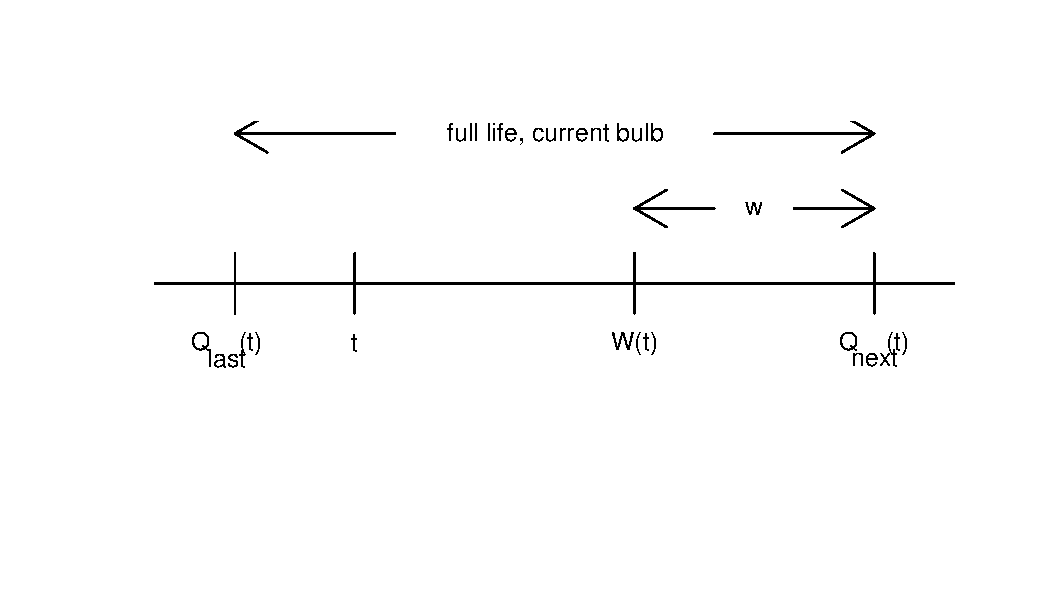
\includegraphics[height=3.0in,width=5.0in]{ResidLife.pdf}

The definition of W(t) sounds complicated, but it is merely saying this:
Looking at the picture, start at $Q_{next}(t)$ and move your eyes
leftward a distance w, but no further leftward than $Q_{last}(t)$.  The
place where you end up is defined to be W(t).

Though W(t) is shown in the picture as being to the right of t, the
opposite could be true.  In fact,

\begin{equation}
\label{diffq}
D(t) \leq w \textrm{ if and only if } W(t) \leq t
\end{equation}

Our goal is to find

\begin{equation}
\lim_{t \rightarrow \infty} P[D(t) \leq w]
\end{equation}

But (\ref{diffq}) shows that

\begin{equation}
\label{3limits}
\lim_{t \rightarrow \infty} P[D(t) \leq w] = 
\lim_{t \rightarrow \infty} P[W(t) \leq t] =
\textrm{ long-run fraction of the time $W(t) \leq t$ as $t \rightarrow
\infty$} 
\end{equation}

(Existence of that long-run fraction as a constant can be shown
mathematically to imply that the limiting probability exists and is
equal to that constant.  But the result is intuitively clear.)

Now let's evaluate the far right-hand side of (\ref{3limits}).  For each
light bulb, let Z(t) the length of the portion of its lifetime to the
right of W(t), i.e.

\begin{equation}
Z(t) = Q_{next}(t) - W(t)
\end{equation}

and let Y(t) be the portion to the left of W(t).  Then:

\begin{equation}
\label{covered}
W(t) \leq t \textrm{ if and only if t is in the interval covered by Z(t)} 
\end{equation}

The Ys and Z form an alternating renewal process as we move from bulb to
bulb.  Thus from Equations (\ref{altoff}), (\ref{3limits}) and
(\ref{covered}) we have that 

\begin{eqnarray}
\lim_{t\rightarrow \infty }P(D(t)\leq w) & = & \frac{E(Z)}{E(Y)+E(Z)}\label{limrt} \\
 & = & \frac{E[\min(L,w)]}{E(L)}
\end{eqnarray}

where L is the lifetime of a bulb.

By Lemma \ref{reverse} we have 

\begin{equation}
E[\min(L,w)]=\int ^{\infty }_{0}P[\min(L,w)>u]\, du=\int ^{w}_{0}P(L>u)\,
du=\int ^{w}_{0}[1-F_{L}(u)]\, du
\end{equation}

since $P[\min(L,w) > u] = 0$ whenever $u > w$.

Substituting this into (\ref{limrt}), and taking derivatives with
respect to w, we have that 

\begin{equation}
\label{resid}
\lim_{t\rightarrow \infty }f_{D(t)}(w)=\frac{1-F_{L}(w)}{E(L)}
\end{equation}

This is a classic result, of central importance and usefulness, as seen
in our upcoming examples later in this section.

\subsection{Age Distribution}
\label{agedistribution}

Analogous to the residual lifetime D(t), let A(t) denote the
\textbf{age} (sometimes called the \textbf{backward recurrence time}) of
the current light bulb, i.e.  the length of time it has been in service.
(In the bus-paradox example, A(t) would be the time which has elapsed
since the last arrival of a bus, to the current time t.) Using an
approach similar to that taken above, one can show that

\begin{equation}
\label{age}
\lim_{t\rightarrow \infty }f_{A(t)}(w)=\frac{1-F_{L}(w)}{E(L)}
\end{equation}

In other words, A(t) has the same long-run distribution as D(t)!

Here is a derivation for the case in which the $L_i$ are discrete.
Remember, our fixed observation point t is assumed large, so that the
system is in steady-state.  Let W denote the lifetime so far for the
current bulb.  Then we have a Markov chain in which our state at any
time is the value of W.  Say we have a new bulb at time 52.  Then W is 0
at that time.  If the total lifetime turns out to be, say, 12, then W
will be 0 again at time 64.  

Let's find the transition probabilities.  First note that when we are in
state i, i.e. $W = i$, we know that the current bulb's lifetime is at
least i+1.  If its lifetime is exactly i+1, our next state will be 0.
So,

\begin{equation}
p_{i,0} = P(L = i+1 | L > i) = \frac{p_L(i+1)}{1-F_L(i)}
\end{equation}

\begin{equation}
p_{i,i+1} = \frac{1-F_L(i+1)}{1-F_L(i)}
\end{equation}

Define

\begin{equation}
q_i = \frac{1-F_L(i+1)}{1-F_L(i)}
\end{equation}

and write

\begin{equation}
\label{rc}
\pi_{i+1} = \pi_i q_i
\end{equation}

Applying (\ref{rc}) recursively, we have

\begin{equation}
\label{telescope}
\pi_{i+1} = \pi_0 q_i q_{i-1}) \cdots q_0 
\end{equation}

But the right-hand side of (\ref{telescope}) telescopes down to

\begin{equation}
\pi_{i+1} = \pi_0 [1 - F_L(i+1) ]
\end{equation}

Then

\begin{equation}
1 = \sum_{i=0}^{\infty} \pi_i 
= \pi_0 \sum_{i=0}^{\infty} [1 - F_L(i)]  
= \pi_0 E(L)
\end{equation}

by (\ref{reverse}). 

Thus

\begin{equation}
\label{piage}
\pi_i =  \frac{1 - F_L(i+1)} {EL}
\end{equation}

in analogy to (\ref{age}).

\subsection{Mean of the Residual and Age Distributions}

Taking the expected value of (\ref{resid}) or (\ref{age}), we get a
double integral.  Reversing the order of integration, we find that
the mean residual life or age is given by

\begin{equation}
\label{variancecounts}
\frac{E(L^2)}{2EL} 
\end{equation}

\subsection{Example:  Estimating Web Page Modification Rates}

My paper, Estimation of Internet File-Access/Modification Rates, {\it
ACM Transactions on Modeling and Computer Simulation}, 2005, 15, 3, 233-253,    
concerns the following problem.  

Suppose we are interested in the rate of modfication of a file in some
FTP repository on the Web.  We have a spider visit the site at regular
intervals.  At each visit, the spider records the time of last
modification to the site.  We do not observe how MANY times the site was
modified.  The problem then is how to estimate the modification rate
from the last-modification time data that we do have. 

I assumed that the modifications follow a renewal process.  Then the
difference between the spider visit time and the time of last
modfication is equal to the age A(t).  I then applied a lot of renewal
theory to develop statistical estimators for the modfication rate.  

\subsection{Example:  The (S,s) Inventory Model Again}
\label{dip}

Here I extend Ross' example that we saw in Section \ref{ross}.

When an order causes the inventory to go below s, we must dip into our
reserves to fill it.  Let R be the amount of reserves we must draw upon.
Assuming that we always have sufficient reserves, what is the
distribution of R?

Recall the renewal process $\tilde{N}(t)$ in Section \ref{ross}.  Then
the distribution of R is that of the residual life for the process
$\tilde{N}(t)$, given approximately by (\ref{resid}).

Suppose for instance that S = 20.0, s = 2.5 and $f_O(x) = 2x$ for $0 < x
< 1$.\footnote{Actually, the values of S and s do not matter here,
though of course the larger S-s is, the better the approximation.}  Then 
from (\ref{variancecounts}),

\begin{equation}
ER = \frac{E(O^2)}{2EO} = \frac{3}{8} 
\end{equation}

\subsection{Example:  Disk File Model}

Suppose a disk will store backup files.  We place the first file in the
first track on the disk, then the second file right after the first in
the same track, etc.  Occasionally we will run out of room on a track,
and the file we are placing at the time must be split between this track
and the next.  Suppose the amount of room X taken up by a file (a
continuous random variable in this model) is uniformly distributed
between 0 and 3 tracks.  

Some tracks will contain data from only one file.  (The file may extend
onto other tracks as well.)  Let's find the long-run proportion of
tracks which have this property.  

Think of the disk as consisting of a Very Long Line, with the
end of one track being followed immediately by the beginning of the next
track.  The points at which files begin then form a renewal process,
with ``time'' being distance along the Very Long Line.  If we observe
the disk at the end of the $k^{th}$ track, this is observing at ``time''
k.  That track consists entirely of one file if and only if the ``age''
A of the current file---i.e. the distance back to the beginning of that
file---is greater than 1.0.

Then from Equation (\ref{age}), we have

\begin{equation}
f_A(w) = \frac{1-\frac{w}{3}}{1.5} = \frac{2}{3} - \frac{2}{9} w
\end{equation}

Then

\begin{equation}
P(A > 1) = \int_{1}^{3} \left (\frac{2}{3} - \frac{2}{9} w \right) ~ dw
= \frac{4}{9}
\end{equation}

\subsection{Example:  Event Sets in Discrete Event Simulation
(difficult)}

Discrete event simulation involves systems whose states change in a
discrete rather than a continuous manner.  For example, the number of
packets currently waiting in a network router changes discretely, while
the air temperature in a weather model changes continuously.

A discrete event simulation program must maintain an {\bf event set},
which is a data structure containing all the pending events.  To make
this concrete, suppose we are simulating a k-server queue.\footnote{For
the details, using the SimPy language, see my introduction to
discrete event simulation, at
\url{http://heather.cs.ucdavis.edu/~matloff/156/PLN/DESimIntro.pdf}.}
There are two kinds of events---job service completions and customer
arrivals.  Since we have k servers, at any time in the simulation we
could have as many as k+1 pending events.  If k = 2, for instance, our
event set could be, say, consist of a service completion for Machine 1
at time 124.3, one for Machine 2 at 95.4, and a customer arrival at time
99.0.

The core of the program consists of a main loop that repeatedly loops
through the following:

\begin{itemize}

\item [(a)] Delete the earliest member of the event set.

\item [(b)] Update simulated time to the time for that event.

\item [(c)] Generate a new event triggered by the one just executed.

\item [(d)] Add the new event to the event set.

\end{itemize}

In our k-server queue example, say the event in (a) is a service
completion.  Then if there are jobs waiting in the queue, this will
trigger the start of service for the new job at the head of the queue,
in (c).

Due to (a), the event list is a priority queue, and thus any of the
wealth of data structures for priority queues could be used to implement
it.  Here we will assume the simplest one, a linear linked list, which
is always maintained in sorted order.

The question is this:  In (d) above, we need to search the list to
determine where to insert our new event in order to enhance our
program's run speed.  Should we start our search at the head of the list
or at its tail?  

An answer to this question was provided in an old paper: On the
Distribution of Event Times for the Notices in a Simulation Event List,
Jean Vaucher, {\it INFOR}, June 1977.  Vaucher realized that this
problem was right up renewal theory's alley.  Our presentation here is
adapted from that paper.

First, think of all events that are ever generated during the entire
simulation.  They comprise the renewal process.  Let $L_i$ denote the
(simulated) time between the $(i-1)^{st}$ and $i^{th}$ events.

Let $t_c$ denote the time of the event in (a), and let $t_d$ denote
earliest time in the event list {\it after} step (a) is performed.  Let
L denote the duration of the event generated in (c), so that that
event's simulated occurrence time will be $t_c + L$.

We will assume that the the size of the event list stays constant at r.
(This is true for many simulations, and approximately true for many
others.) Now, the question of where in the event list to place our new
event is equivalent to asking how many events in the list have their
times $t_e$ after $t_c+L$.  That in turn is the same as asking how many
of the events have a residual life Z of greater than L.  Call that number
$K$.  

The quantity of interest is 

\begin{equation}
\gamma = \frac{E(K)}{r}
\end{equation}

If $\gamma < 0.5$ we should start our search at the head of the list;
otherwise we should start at the tail.

So, let's derive E(K).  First write

\begin{equation}
\label{tot}
E(K) = E [ E(K|L) ]
\end{equation}

To simplify notation, let g denote the residual life density
(\ref{resid}).  Then, using the point above concerning residual life
and keeping in mind that L is a ``constant' in our conditional
computation here, we have

\begin{equation}
E(K|L) = r P(Z > L) 
= r \cdot \int_{L}^{\infty} g(t) ~ dt
\end{equation}

Now use this in (\ref{tot}):

\begin{equation}
E(K) = r \int_{0}^{\infty} 
\left ( \int_{s}^{\infty} g(t) ~ dt \right )
f_L(s) ~ ds
\end{equation}

One then does an integration by parts, making use of the fact that
$g\prime (z) = -\frac{f(x)}{E(L)}$.  After all the dust clears, it turns
out that 

\begin{equation}
\gamma = 1 - E(L) \int_{0}^{\infty} g^2(t) ~ dt
\end{equation}

In Vaucher's paper, he then evaluated this expression for various
distributions of L, and found that for most of the distributions he
tried, $\gamma$ was in the 0.6 to 0.8 range.  In other words, one
typically should start the search from the tail end.

\subsection{Example: Memory Paging Model}
\label{mem} 

(Adapted from \textit{Probabiility and Statistics, with Reliability, Queuing
and Computer Science Applicatiions}, by K.S. Trivedi, Prentice-Hall,
1982 and 2002.)

Consider a computer with an address space consisting of n pages, and a program
which generates a sequence of memory references with addresses (page numbers)
$D_{1},\, D_{2},\, ...$ In this simple model, the $D_{i}$ are assumed
to be i.i.d. integer-valued random variables.

For each page i, let $T_{ij}$ denote the time at which the $j^{th}$
reference to page i occurs. Then for each fixed i, the $T_{ij}$ form a
renewal process, and thus all the theory we have developed here
applies.\footnote{Note, though, tht all random variables here are
discrete, not continuous.} Let $F_{i}$ be the cumulative distribution
function for the interrenewal distribution, i.e. $F_{i}(m)=P(L_{ij} \leq m)$,
where $L_{ij}=T_{ij}-T_{i,j-1}$ for m = 0, 1, 2, ...

Let $W(t,\tau )$ denote the working set at time t, i.e. the
collection of page numbers of pages accessed during the time $(t-\tau
,t)$, and let $S(t,\tau )$ denote the size of that set. We are
interested in finding the value of

\begin{equation}
s(\tau )=\lim_{t\rightarrow \infty } E[S(t,\tau )]
\end{equation}

Since the definition of the working set involves looking backward \(
\tau $ amount of time from time t, a good place to look for an
approach to finding $s(\tau )$ might be to use the limiting
distribution of backward-recurrence time, given by 
Equation (\ref{piage}). 

Accordingly, let $A_{i}(t)$ be the age at time t for page i. Then

\begin{quote}
Page i is in the working set if and only if it has been accessed 
after time $t-\tau $., i.e. $A_{i}(t)<\tau $.  
\end{quote}

Thus, using (\ref{piage}) and letting $1_{i}$ be 1 or 0 according to
whether or not $A_{i}(t)<\tau $, we have that

\begin{eqnarray}
s(\tau ) & = & \lim_{t\rightarrow \infty } E(\sum ^{n}_{i=1}1_{i})
\nonumber \\
 & = & \lim_{t\rightarrow \infty } \sum ^{n}_{i=1}P(A_{i}(t)<\tau )
 \nonumber \\
 & = & \sum ^{n}_{i=1}\sum ^{\tau -1}_{j=0}\frac{1-F_{i}(j)}{E(L_{i})}
\end{eqnarray}

\startproblemset

\oneproblem
Consider a renewal process in which lifetimes have the values
1, 2, 3 or 4, with probability 1/4 each.

\begin{itemize}

\item [(a)] Find P[N(3) = 2].

\item [(b)] For large integer t, find the probability that the current
renewal period began at t-2.

\end{itemize}

\oneproblem
Suppose the burn time for light bulbs is normally distributed with 
mean 100.0 and variance 225, and consider the associated renewal 
process (the lamp's bulb is replaced as soon as it burns out). Find 
$P[ N(500) \geq 4]$.  

\oneproblem
Consider a renewal process in which lifetimes have the values
1, 2, 3 or 4, with probability 1/4 each.  Express your answers as single
fractions, e.g. 25/6 (not as decimal numbers or numerical algebraic
expressions).

\begin{itemize}

\item [(a)] Find P[N(3) = 2].

\item [(b)] For large integer t, find the probability that the current
renewal period began at t-2.

% \item [(c)] Suppose the lifetimes are continuous random variables, with
% a uniform distribution on (0,1).  Give a numerical expression for the
% density of $R_2$.

\end{itemize}


